\chapter{Arhitektura i dizajn sustava}
		\texttt{}{ Arhitekturu projektnog sustava možemo podijeliti u 3 cjeline:}
	\begin{itemize}
		\item 	\textit{Web aplikacija }
		\item 	\textit{Web poslužitelj}
		\item 	\textit{Baza podataka }		
	\end{itemize}


                \texttt{}{
             Web preglednik je dio arhitekture koji korisniku omogućuje pregled web stranice i svih sadržaja na njoj. Svaki internetski preglednik je prevoditelj. Korisnik putem web preglednika šalje zahtjev web poslužitelju. 
            }

            
                \texttt{}{
             Web poslužitelj osnova je rada web aplikacije. Njegov primaran zadatak je komunikacija klijenta s aplikacijom. Komunikacija se odvija preko HTTP (engl. Hyper Text Transfer Protocol) protokola, sto je protokol u prijenosu informacija na webu. Poslužitelj je onaj koji pokreće web aplikaciju te joj prosljeđuje zahtjev
            }


            
                \texttt{}{
            Korisnik koristi web aplikaciju za obrađivanje željenih zahtijeva. Web aplikacija obrađuje zahtjev te ovisno o zahtjevu, pristupa bazi podataka nakon čega preko poslužitelja vraća korisniku odgovor u obliku HTML dokumenta vidljivog u web pregledniku.}
               

                \texttt{}{
             Null grupa 2022./2023. za projekt na predmetu Programsko inženjerstvo 2022./2023. odabrala je AngularJS sustav za izradu projetknog zadatka. 
            Arhitektura AngularJS-a temelji se na MVC dizajnu (Model, view, controller).
            Model View Controller ili MVC kako se popularno naziva, uzorak je dizajna softvera za razvoj web aplikacija. MVC dizajn sastoji se od sljedeća tri dijela:
            }
            \begin{itemize}
		\item 	\text{ Model je najniža razina uzorka odgovornog za održavanje podataka. }
		\item 	\text{ Prikaz(view) odgovoran je za prikazivanje svih ili dijela podataka korisniku.}
		\item 	\text{Kontroler je softverski kod koji kontrolira interakcije između modela i prikaza.}		
	\end{itemize}
        \eject

             \begin{figure}[H]
			            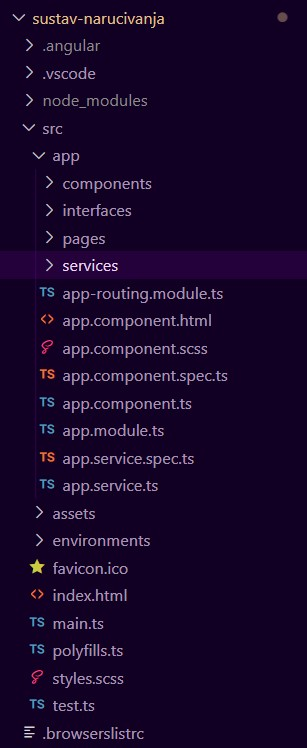
\includegraphics[width=50mm, height= 125mm]{slike/arh.jpg} %veličina u odnosu na širinu linije
			            \caption{Struktura implementacije aplikacije iz VSC.}
			            \label{fig:promjene2} %label mora biti drugaciji za svaku sliku
		            \end{figure}

              
               \texttt{}{ Aplikaciju smo rastavili na komponente, sučelja, stranice i servise. 
               Komponente su implementirani dijelovi stranice koje možemo ubaciti kao cjelinu u neku od pages(stranica) kako ne bismo morali pisati dupli kod. Pages(stranice) su sve stranice u našoj aplikaciji. Svaki "page" sastavljen je od '.html' datoteke za strukturu, '.scss' datoteke za dizajn, '.module.ts' u kojoj možemo Typescriptom napraviti uvoz pojedinog modula Angulara u stranicu, '.spec.ts' u kojoj definiramo pojedine funkcije i '.ts' u kojoj definiramo putanje i povezivanje svih dokumenata.
               
               }
        
               \texttt{}{
               Razvojno okruženje koje će koristiti programeri Null grupe će biti Visual Studio Code. Za izradu i doradu koda programeri koriste GitLab sustav.
            Za razvoj dokumentacije grupa će koristiti Overleaf aplikaciju radi sistematičnosti izrade.
               }
            
               %\includegraphics[width=\textwidth{slike/mvc.jpeg}
               
		\section{Baza podataka}
			
			\textbf{\textit{dio 1. revizije}}\\
			
		{PostgresSQL baza podataka sastoji se od 7 tablica. Entitet users je supertip koji se disjointed grana na četiri tablice: admin, patient, doctor i nurse. Primarni ključ svih tih entiteta je ID koji se u tablici user automatski generira. Tablica patient također sadrži strani ključ doctorid, jer je pacijent pri registraciji obavezan izabrati svog liječnika. Tablica nurse ima strani ključ teamName, referencu na tablicu team, jer u jednom timu kojeg administrator određuje može raditi više medicinskih tehničara. Također ta vrijednost može biti null jer tehničar ne mora nužno biti dio tima. Osim tih tablica također baza podataka sadrži već prije spomenutu tablicu team te appointment. Primarni ključ teama je teamName, a također i sadrži strani ključ doctorid, referencu na tablicu doctor, u kojoj je naveden id liječnika dodjeljenog timu. Tablica appointment sadrži primarni ključ appointmentId koji se automatski generira te tri strana ključa. Patientid koji obavezno nije null, referenca na pacijenta koji dolazi na pregled. Druga dva strana ključa doctorId i nurseId su međusobno isključivi, odnosno ako jedan ima vrijednost, drugi mora biti null, jer pacijent dolazi na pregled ili kod liječnika ili kod tehničara. Pregled je također određen timestampom time, vremenom kad je ugovoren i intervalom duration.}
		
			\subsection{Opis tablica}
			

				\textit{Svaku tablicu je potrebno opisati po zadanom predlošku. Lijevo se nalazi točno ime varijable u bazi podataka, u sredini se nalazi tip podataka, a desno se nalazi opis varijable. Svjetlozelenom bojom označite primarni ključ. Svjetlo plavom označite strani ključ}
				
				
				\begin{longtblr}[
					label=none,
					entry=none
					]{
						width = \textwidth,
						colspec={|X[6,l]|X[6, l]|X[20, l]|}, 
						rowhead = 1,
					} %definicija širine tablice, širine stupaca, poravnanje i broja redaka naslova tablice
					\hline \multicolumn{3}{|c|}{\textbf{users}}	 \\ \hline[3pt]
					\SetCell{LightGreen} ID     &   INT     &  	Jedinstveni id svakog korisnika, generira se automatski, primarni ključ tablice korisnik \\ \hline
					name	& VARCHAR &   Ime korisnika	\\ \hline 
					surname & VARCHAR &  Prezime korisnika \\ \hline 
					 phoneNumber & VARCHAR	&  	Telefonski broj korisnika, jedinstven ta svakog korisnika	\\ \hline 
					 mail & VARCHAR	&  	Adresa elektroničke pošte korisnika, jedinstvena za svakog korisnika	\\ \hline 
					password & VARCHAR	&  	Lozinka korisnika za prijavu u sustav	\\ \hline 
					sex & VARCHAR	&  	spol korisnika	\\ \hline 
					dateOdBirth & DATE	&  	Datum rođenja korisnika	\\ \hline 
				\end{longtblr}
				
				\begin{longtblr}[
					label=none,
					entry=none
					]{
						width = \textwidth,
						colspec={|X[6,l]|X[6, l]|X[20, l]|}, 
						rowhead = 1,
					} %definicija širine tablice, širine stupaca, poravnanje i broja redaka naslova tablice
					\hline \multicolumn{3}{|c|}{\textbf{admin}}	 \\ \hline[3pt]
					\SetCell{LightGreen} adminid     &   INT     &  	Strani ključ, referenca na id u tablici users \\ \hline
				\end{longtblr}
				
			\begin{longtblr}[
					label=none,
					entry=none
					]{
						width = \textwidth,
						colspec={|X[12,l]|X[6, l]|X[20, l]|}, 
						rowhead = 1,
					} %definicija širine tablice, širine stupaca, poravnanje i broja redaka naslova tablice
					\hline \multicolumn{3}{|c|}{\textbf{patient}}	 \\ \hline[3pt]
					numberOfMissedApp   &   INT & Broj ugovorenih pregleda koje je pacjent propustio \\ \hline
					\SetCell{LightGreen} patientid     &   INT     &  	Strani ključ, referenca na id u tablici users \\ \hline
					\SetCell{LightBlue} doctorid & INT & ID doktora kojeg je pacijent izabrao pri registraciji \\ \hline
				\end{longtblr}
			
			
			\begin{longtblr}[
					label=none,
					entry=none
					]{
						width = \textwidth,
						colspec={|X[6,l]|X[6, l]|X[20, l]|}, 
						rowhead = 1,
					} %definicija širine tablice, širine stupaca, poravnanje i broja redaka naslova tablice
					\hline \multicolumn{3}{|c|}{\textbf{doctor}}	 \\ \hline[3pt]
					\SetCell{LightGreen} doctorid      &   INT     &  	Strani ključ, referenca na id u tablici users \\ \hline
				\end{longtblr}
			
			\begin{longtblr}[
					label=none,
					entry=none
					]{
						width = \textwidth,
						colspec={|X[6,l]|X[6, l]|X[20, l]|}, 
						rowhead = 1,
					} %definicija širine tablice, širine stupaca, poravnanje i broja redaka naslova tablice
					\hline \multicolumn{3}{|c|}{\textbf{nurse}}	 \\ \hline[3pt]
					\SetCell{LightGreen} nurseid     &   INT     &  	Strani ključ, referenca na id u tablici users \\ \hline
					\SetCell{LightBlue}teamName & VARCHAR & Ime tima kojem je medicinska sestra dodjeljena, može biti null \\\hline
				\end{longtblr}
				
				\begin{longtblr}[
					label=none,
					entry=none
					]{
						width = \textwidth,
						colspec={|X[6,l]|X[6, l]|X[20, l]|}, 
						rowhead = 1,
					} %definicija širine tablice, širine stupaca, poravnanje i broja redaka naslova tablice
					\hline \multicolumn{3}{|c|}{\textbf{team}}	 \\ \hline[3pt]
					\SetCell{LightGreen} teamName      &   VARCHAR     &  	Ime tima \\ \hline
					\SetCell{LightBlue}doctorid & INT & Strani ključ, ID doktora koji radi u timu \\\hline
				\end{longtblr}
			
			\begin{longtblr}[
					label=none,
					entry=none
					]{
						width = \textwidth,
						colspec={|X[10,l]|X[6, l]|X[20, l]|}, 
						rowhead = 1,
					} %definicija širine tablice, širine stupaca, poravnanje i broja redaka naslova tablice
					\hline \multicolumn{3}{|c|}{\textbf{appointment}}	 \\ \hline[3pt]
					\SetCell{LightGreen} appointmentId       &   INT     &  	Jedinstveni ID pregleda, generira se automatski \\ \hline
					\SetCell{LightBlue}patientid & INT & Strani ključ, ID pacijenta koji je zakazao pregled, ne može biti null \\\hline
					\SetCell{LightBlue}doctorid & INT & Strani ključ, ID doktora koji koji vrši pregled\\\hline
					\SetCell{LightBlue}nurseid & INT & Strani ključ, ID medicinskog tehničara koji vrši pregled \\\hline
					time & TIMESTAMP & Vrijeme u koje je pregled ugovoren \\ \hline
					duration & INTERVAL & Trajanje pregleda \\ \hline
				\end{longtblr}
			
			
			\subsection{Dijagram baze podataka}
				\begin{figure}[H]
			            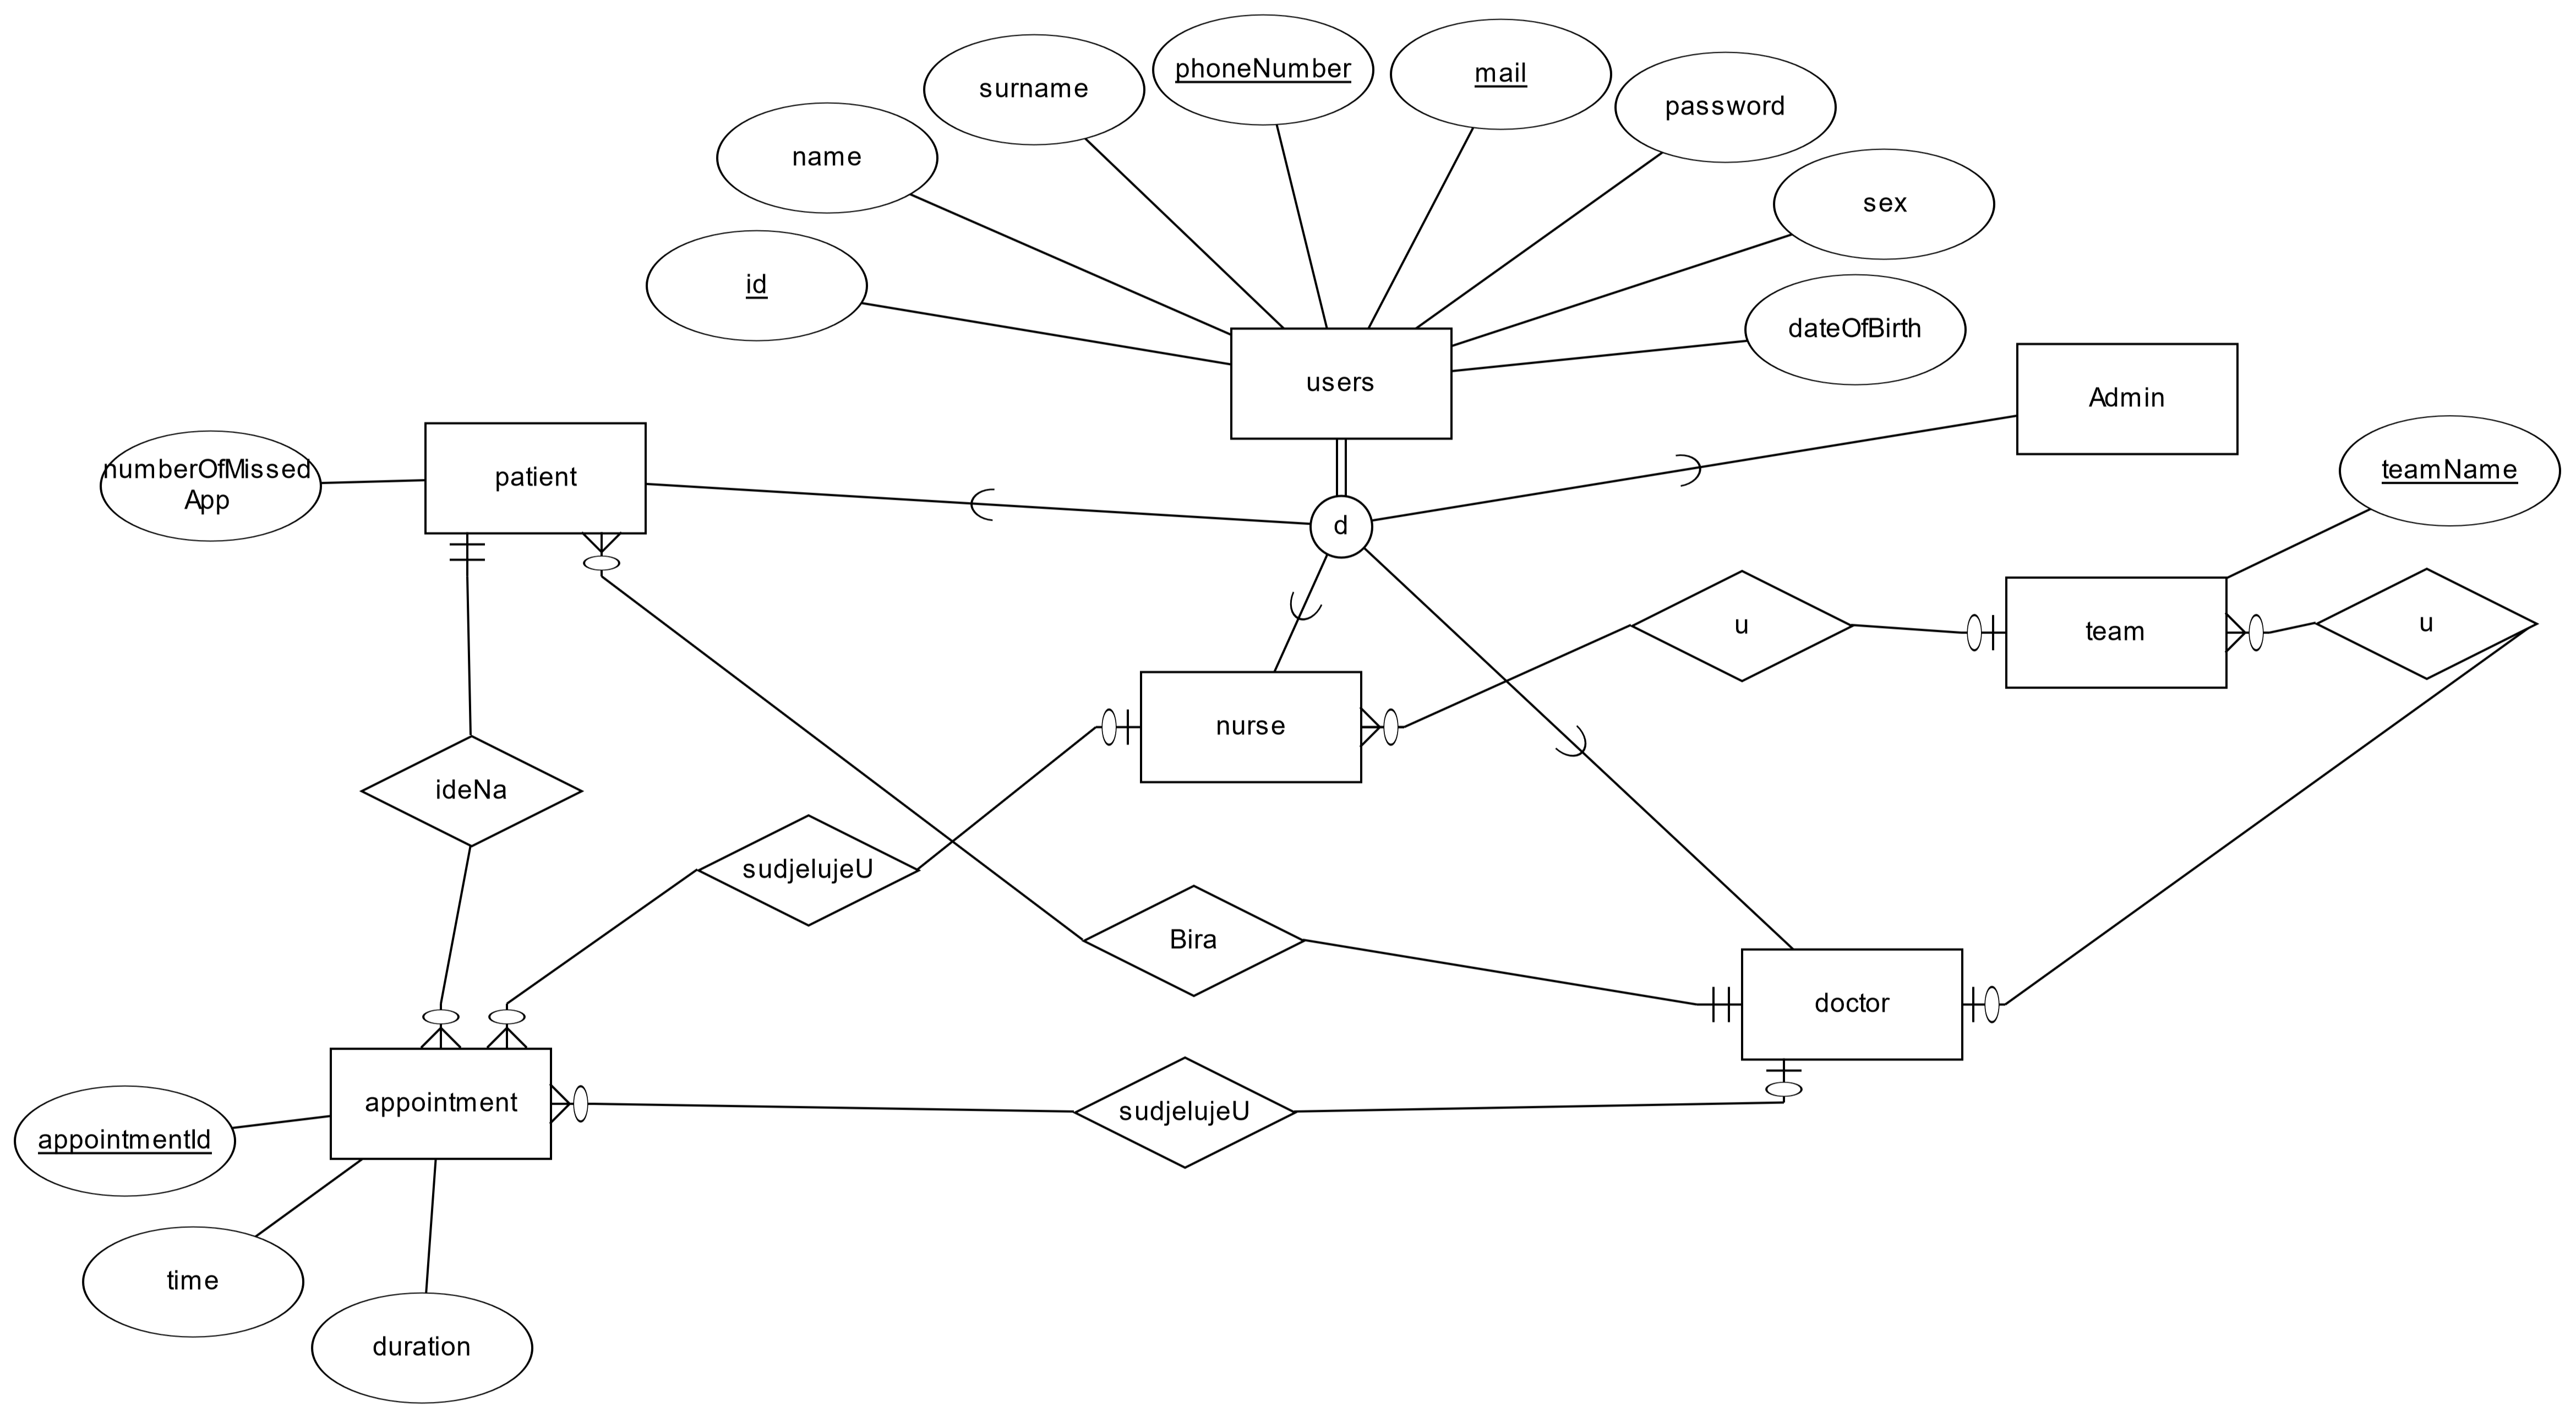
\includegraphics[width=\textwidth]{slike/BAZA_er.png} %veličina u odnosu na širinu linije
			            \caption{ER dijagram baze podataka}
			            \label{fig:promjene2} %label mora biti drugaciji za svaku sliku
		            \end{figure}			
			\subsection{Dijagram baze podataka}
				\begin{figure}[H]
			            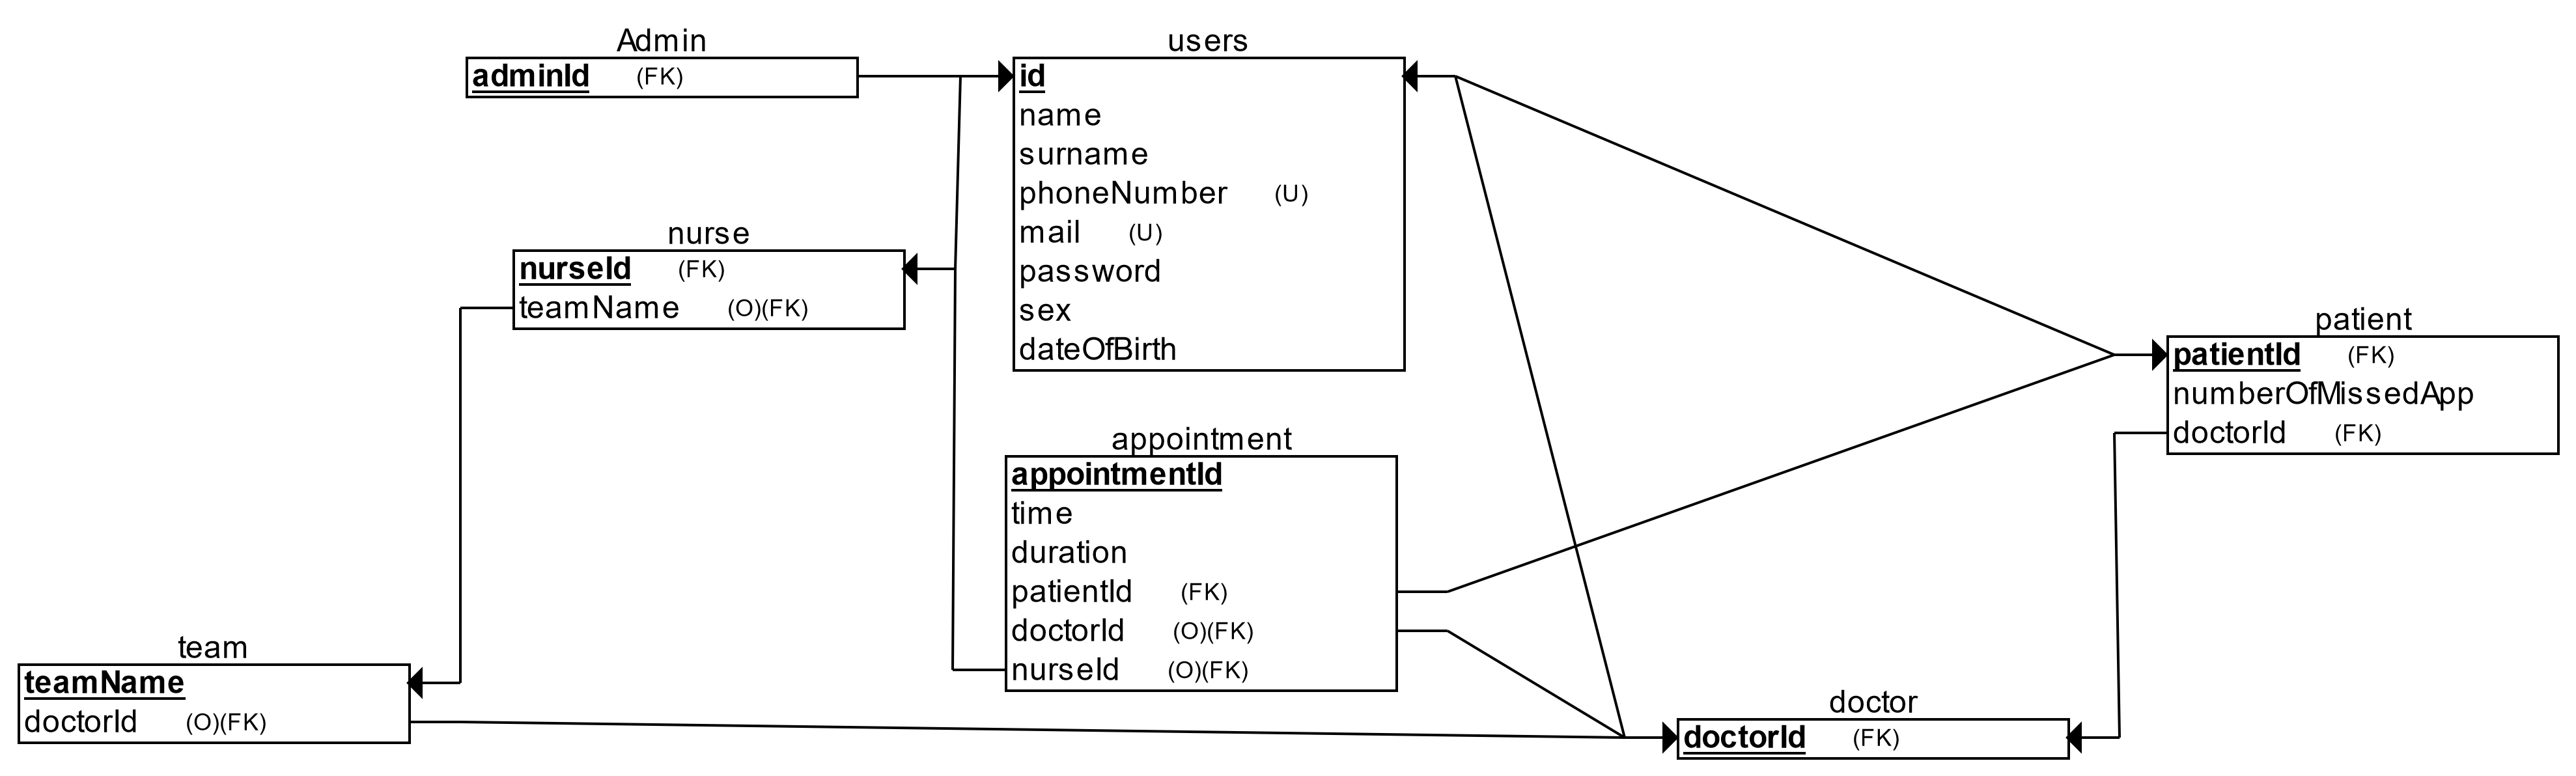
\includegraphics[width=\textwidth]{slike/BAZA_racionalni.png} %veličina u odnosu na širinu linije
			            \caption{Racionalni dijagram baze podataka}
			            \label{fig:promjene2} %label mora biti drugaciji za svaku sliku
		            \end{figure}
		            
			
			\eject
			
			
		\section{Dijagram razreda}
		
			%\textit{Potrebno je priložiti dijagram razreda s pripadajućim opisom. Zbog preglednosti je moguće dijagram razlomiti na više njih, ali moraju biti grupirani prema sličnim razinama apstrakcije i srodnim funkcionalnostima.}\\
			
			%\textbf{\textit{dio 1. revizije}}\\
			
			%\textit{Prilikom prve predaje projekta, potrebno je priložiti potpuno razrađen dijagram razreda vezan uz \textbf{generičku funkcionalnost} sustava. Ostale funkcionalnosti trebaju biti idejno razrađene u dijagramu sa sljedećim komponentama: nazivi razreda, nazivi metoda i vrste pristupa metodama (npr. javni, zaštićeni), nazivi atributa razreda, veze i odnosi između razreda.}\\
			
			Na slici 4.3 prikazan je dijagram razreda koji pripada backend dijelu arhitekture. Razredi iz dijagrama predstavljaju strukturu baze podataka u aplikaciji te svaki razred predstavlja jedan entitet iz baze. Metode koje su implementirane komuniciraju s bazom podataka, ako je potrebno, upisuju odgovarajuće podatke u bazu ili ih vraćaju iz baze. Razred User predstavlja svakog korisnika aplikacije i koji može koristiti određene funkcionalnosti sustava. Međutim, prije toga se mora registrirati s osobnim podacima: ime, prezime, spol, broj telefona, e-mail, lozinka i datum rođenja. Razred Pacijent predstavlja korisnika koji je registriran kao pacijent i ima pristup svojim terminima uz funkcionalnosti zakazivanja i otkazivanja termina, kojeg predstavlja razred Appointment. Nešto veću ovlast ima medicinska sestra koju predstavlja razred Nurse, ona može i unaprijed definirati termine usluga. Razred Doctor predstavlja liječnika koji može definirati slobodne termine pregleda, ali i definirati pravila za naručivanje. Najvišu ovlast ima administrator, kojeg predstavlja razred Admin. On može stvarati timove, koje predstavlja razred Teams, te upisati nove liječnike i medicinske sestre u bazu.
			
			\begin{figure}[H]
			            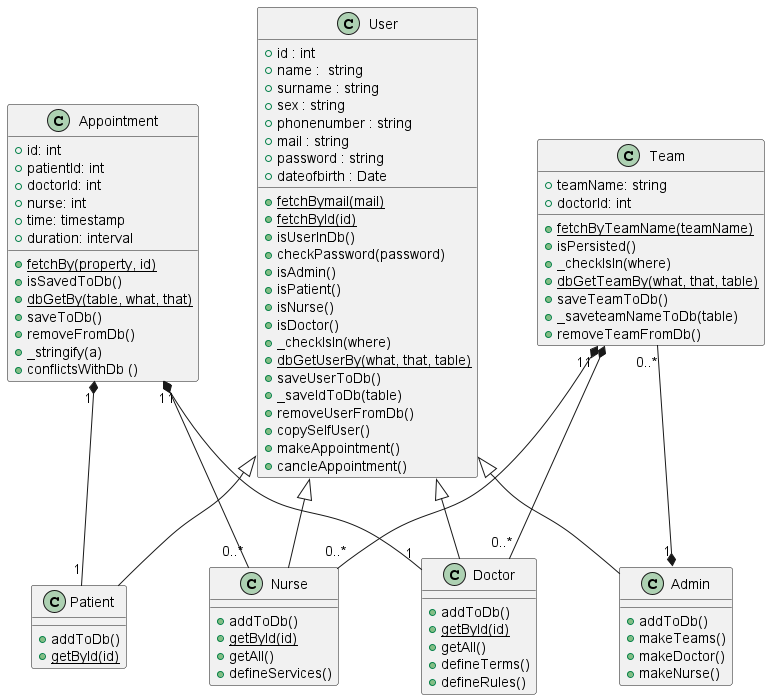
\includegraphics[width=\textwidth]{slike/backend_class_diagram.png} %veličina u odnosu na širinu linije
			            \caption{Dijagram razreda - Modeli}
			            \label{fig:promjene2} %label mora biti drugaciji za svaku sliku
		      \end{figure}
		      
		   \begin{figure}[H]
			            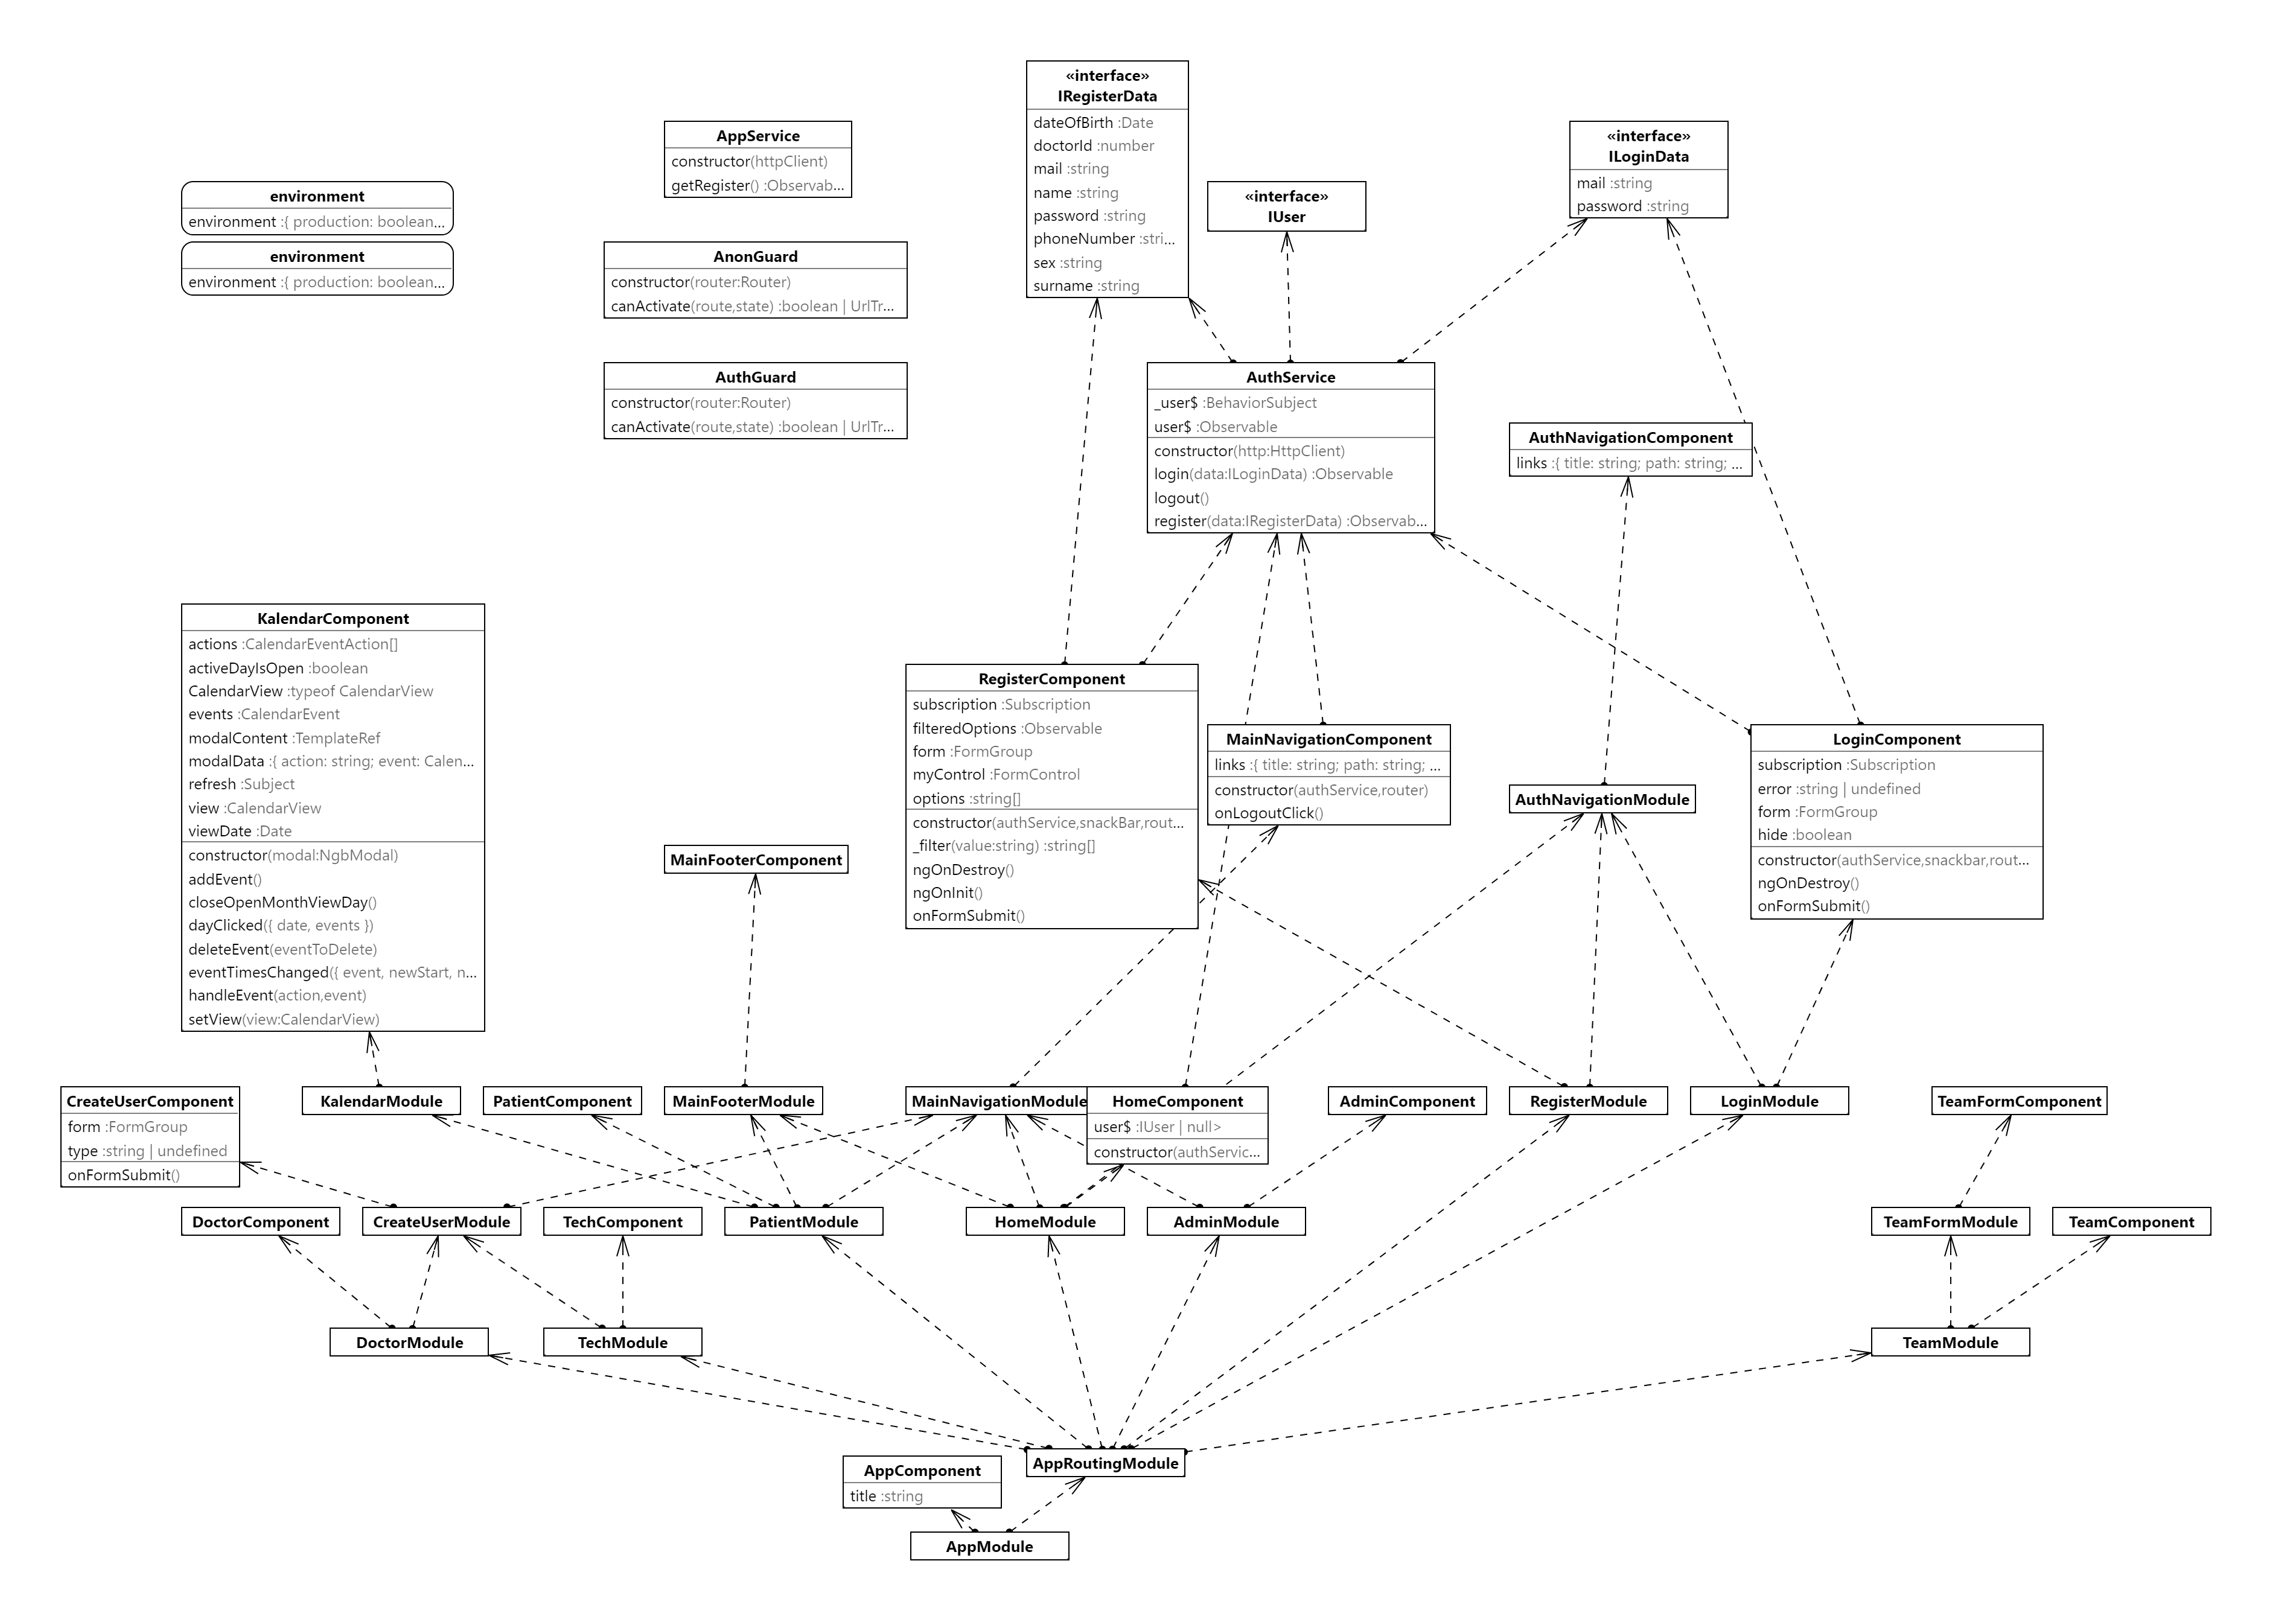
\includegraphics[width=\textwidth]{slike/frontend_class_diagram.png} %veličina u odnosu na širinu linije
			          \caption{Dijagram razreda - frontend}
			            \label{fig:promjene2} %label mora biti drugaciji za svaku sliku
		      \end{figure}
			
		%	\textbf{\textit{dio 2. revizije}}\\			
			
		%	\textit{Prilikom druge predaje projekta dijagram razreda i opisi moraju odgovarati stvarnom stanju implementacije}
			
			
			
		%	\eject
		
		%\section{Dijagram stanja}
			
			
			%\textbf{\textit{dio 2. revizije}}\\
			
			%\textit{Potrebno je priložiti dijagram stanja i opisati ga. Dovoljan je jedan dijagram stanja koji prikazuje \textbf{značajan dio funkcionalnosti} sustava. Na primjer, stanja korisničkog sučelja i tijek korištenja neke ključne funkcionalnosti jesu značajan dio sustava, a registracija i prijava nisu. }
			
			
			%\eject 
		
		%\section{Dijagram aktivnosti}
			
			%\textbf{\textit{dio 2. revizije}}\\
			
			 %\textit{Potrebno je priložiti dijagram aktivnosti s pripadajućim opisom. Dijagram aktivnosti treba prikazivati značajan dio sustava.}
			
			%\eject
		%\section{Dijagram komponenti}
		
			%\textbf{\textit{dio 2. revizije}}\\
		
			 %\textit{Potrebno je priložiti dijagram komponenti s pripadajućim opisom. Dijagram komponenti treba prikazivati strukturu cijele aplikacije.}